For our end goal of enabling large-scale autotuning, we need to explore the current capabilities and limitations of TVM first, especially with regard to the execution of multiple autotuning jobs simultaneously. The modern \gls{dl} landscape is very diverse in terms of models and hardware, so to evaluate TVM in a diverse range of scenarios is crucial for gaining a proper understanding. To this end, we developed a framework that enables us to a large number of experiments rapidly.

\section{SimpleTVM}
Since using TVM follows a similar flow every time, we created SimpleTVM which exposes the individual steps through a convenient interface. This makes it easy for researches who are new to TVM to get started. FSince a lot of the experiments include benchmarking, time measurements are taken for most steps and automatically saved in a \textit{benchmarking context}. The flow of SimpleTVM has some dependencies, which are enforced. For example, a model needs to be imported before building. The interface including possible flows is depicted in Figure \ref{fig:simpletvm-interface}. The methods that are exposes are now regarded closer.

\begin{figure}
	\centering
	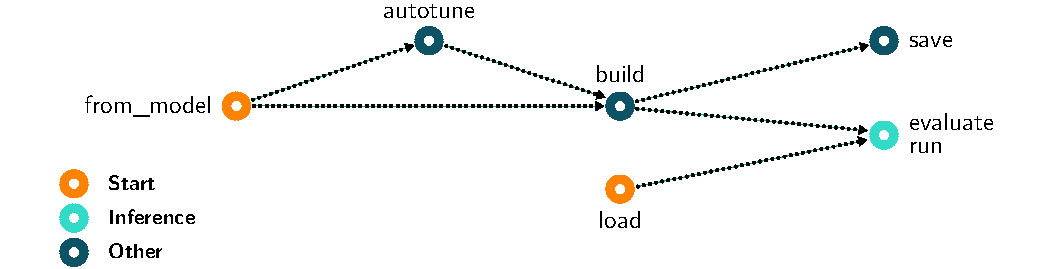
\includegraphics[width=\textwidth]{simpletvm_interface.pdf}%
	\caption{Interface and flow of SimpleTVM}
	\label{fig:simpletvm-interface}
\end{figure}

\begin{description}
	\item[\pythoninline/from_model/] Loading the Relay representation for the model is the beginning of a TVM flow. To that end, TVM supports the import from various frontends. Before the import of the model, however, it needs to be loaded and prepared for import. How exactly this is done differs even inside the same framework. SimpleTVM provides a unified import interface for TVM testing models, TensorFlow saved models (.pb files) and TensorFlow hub models. \pythoninline/from_model/ can easily be extended to support more frontends.
	\item[\pythoninline/autotune/] Once a model has been imported, autotuning can be run for each of the tensor operators. This step is optional, since TVM falls back to a default implementation if no records for that tensor operator exist in the autotuning database. Since this step is rather complex, there is a plethora of configuration options, the most important of which are exposed in \pythoninline/autotune/'s interface. SimpleTVM is designed to get new users started quickly so there are default values, but more experienced users can adjust the values according to their circumstances.
	\item[\pythoninline/build/] Before a TVM model can be executed, the target-specific executable needs to be build from the Relay model as described in the previous chapter. When building, SimpleTVM can either automatically use records from the global autotuning database, or the results from a specific autotuning job can be used.
	\item[\pythoninline/save/] After building, the library containing the operators can be saved along with the graph description and weights.
	\item[\pythoninline/load/] Beyond starting from an imported model, SimpleTVM can also load a previously saved TVM modules, which makes it possible to use a model that has been autotuned earlier. Saved modules can only be loaded if they have been built on the same device.
	\item[\pythoninline/run/] Inference can be run using this method. It accepts and returns a NumPy array. The input can, for example, be an image. However, loading the image and preparing it for inference, e.g., scaling and normalizing, needs to be done by the user.
	\item[\pythoninline/evaluate/] To profile the performance, \pythoninline/evaluate/ runs inference on random data multiple times, then averages the measured times. However, in contrast to the profiling stage of autotuning, not the performance of individual tensor operators but the whole model is measured.
\end{description}

An example of how SimpleTVM is typically used is presented in Listing \ref{lst:simpletvm-flow}. First, the \pythoninline/BenchmarkingContext/ is created (Line 1), which stores information about the current run such as the run id (a 32-character alphanumeric identifier for this execution of SimpleTVM), target device, measured times, the loaded model and the target device key to send to the tracker. When using a CPU as target device, the CPU architecture should be specified so TVM can select the proper hardware-specific tensor instructions. The benchmarking context is passed to the \pythoninline/SimpleTVM/ object (Line 2). Here, the address of the RPC tracker can be specified for distributed autotuning. If the address is not specified, autotuning will create a local tracker and server to perform autotuning on the same device as the client. Next, a model is imported (Line 3). Since the name of the output layer and the size of the output vector differs, it needs to specified explicitly. SimpleTVM's concise, chained syntax is used to autotune, build, save and evaluate the model (Line 4). For the sake of brevity, default parameters are leveraged, but the user can customize the actual calls to TVM functions by providing more parameters. Finally, the benchmarking context is saved (Line 5). This enables analysis at a later point, e.g., to examine the autotuning process or the inference performance measured by the evaluation. Note that this step is distinct from the saving of the TVM module. At a later point and usually by another application, the saved module which is identified by the run id can be loaded back. Then it can be used run inference on any data.

\begin{listing}
\begin{pythoncode}
ctx = BenchmarkingContext('cpu', device_key='i7', cpu_arch='skylake')
tvm = SimpleTVM(ctx, rpc_tracker=('tracker', 9190))
tvm.from_model('mobilenet.pb', output_name='out', output_size=10)
tvm.autotune().build().save().evaluate()
ctx.save()

# Saved model can be used later to run inference
tvm.load('run_id')
prediction = tvm.run(data)
\end{pythoncode}
\unskip
\caption{Typical SimpleTVM flow for CPU including autotuning}
\label{lst:simpletvm-flow}
\end{listing}

Additionally to SimpleTVM, we developed an automated benchmarking script called \textit{superb}. superb is short for \enquote{super benchmark} because it allows testing of different configurations without human intervention, so it performs benchmarking on a higher level than SimpleTVM's mechanisms. The user can specify the values for all parameters that should be tested. superb enumerates all possible combinations, effectively determining the $n$-ary product set of all value lists, then executes SimpleTVM once with each configuration. Additionally, it sets up the required servers and the tracker. The results from all configurations are collected and can then be processed by another script. This script evaluates the resulting inference performances, aggregates some information and writes them into a file, enabling further analysis with other tools such as Jupyter notebooks.

All SimpleTVM-related files are stored in the \enquote{\textasciitilde /.tvm-benchmark} directory. This includes the autotuning databases of currently running jobs, the global autotuning database and a file containing only the best known configurations. There are subdirectories for each SimpleTVM run with a log file for debugging, the saved benchmarking context and the autotuning log file for this run, if applicable. In another subdirectory, the results of superb experiments are collected with a csv file containing the aggregate information like mean autotuning time and the mean execution time for each stage. Finally, all saved modules are saved in a directory named after their run id.

Since we want to test TVM on a variety of machines, we created Docker images to be able to easily deploy TVM with all dependencies on any server. The \gls{gpu} version also includes the CUDA libraries, and a helper script for using the images mounts some folders into the container and sets up the environment. The Docker images in conjunction with SimpleTVM and superb form the foundation for our experiments.

\section{Parameters}
Autotuning with TVM offers a plethora of configuration options that affect both the autotuning process itself and the result. Setting these parameters to adequate values for the given job and hardware requires knowledge of how TVM works, but in some cases it is a matter of trial and error. However, guidelines and descriptions of the most important parameters can help. All of the following parameters can be specified when using SimpleTVM
\begin{description}
	\item[Number of trials] This determines the number of configurations to try for each autotuning task. A higher number will generally result in a better inference performance since the search space can be explored more, but this results in an increased autotuning completion time. However, the result starts to converge to the optimum after about 500 iterations, so there is a limit to the inference performance that can be achieved. Especially with CPUs, that have a small search space compared to \glspl{gpu}, there might not even be more options to try. Practically, the optimal result can be expected with the number of trials set to 2000.
	\item[Profiling timeout] This determines the time after which the profiling for one configuration is killed if it runs too long. Since every tensor operator has a different computational intensity and performance varies across types of hardware, this timeout needs to be adjusted accordingly. A high profiling timeout will allow longer execution, which drives up total autotuning completion time and might not yield better results since long-running implementations are not good and can safely be killed. A low profiling timeout might also kill of good implementations. It should be noted that the optimal timeout does not depend on the actual execution time, since profiling runs the implementation multiple times and might even dynamically adjust the number of executions. In practice, a low timeout should be set first. If the log shows too many timeout errors, the timeout can be increased. 5 seconds seems to be a good value for \gls{gpu} target devices, while 20 seconds or more are appropriate for CPU autotuning.
	\item[Batch size] This determines how many configurations are selected and built in parallel for every autotuning iteration. This can speed up autotuning considerably, especially if a large number of CPU cores are available on the client to run many compiler processes in parallel. The number of cores is also the default value. For larges batches, the model is updated and queried less frequently, but in general there seems to be no detrimental effect of having a high batch size. It should be notes that this is not the same as the batch size of the model, which would change the shape of the tensor operators.
	\item[Transfer learning] This determines whether or not transfer learning is used between jobs. According to this setting, the data from the global autotuning database might be used to train the cost model at the start of each task. Between tasks, there is always transfer learning. Usually, transfer learning should be enabled for the most optimal inference performance results. However, we disable transfer learning for experiments to guarantee a fair comparison between earlier and later ones.
\end{description}


\section{Capabilities}
Using SimpleTVM and our knowledge about proper parameter settings as foundation, we evaluated how TVM performs in comparison to state-of-the-art manual tensor operator libraries. We use TensorFlow 1.14 as baseline since it is a popular framework for \gls{dl} applications. cuDNN is enabled for \gls{gpu}. Autotuning with TVM was executed with 2000 trials, so the numbers should represent the optimal implementation. For evaluation, we test a Mobilenet with a batch size of one on two mobile-grade CPUs (Intel Core i5-5300U and i5-7300U), a server-grade CPU (Intel Xeon E5-2650 v3) and a high-end \gls{gpu} (NVIDIA Tesla K80). The same two images were used as model input in all cases.

\begin{figure}[h]
	\centering
	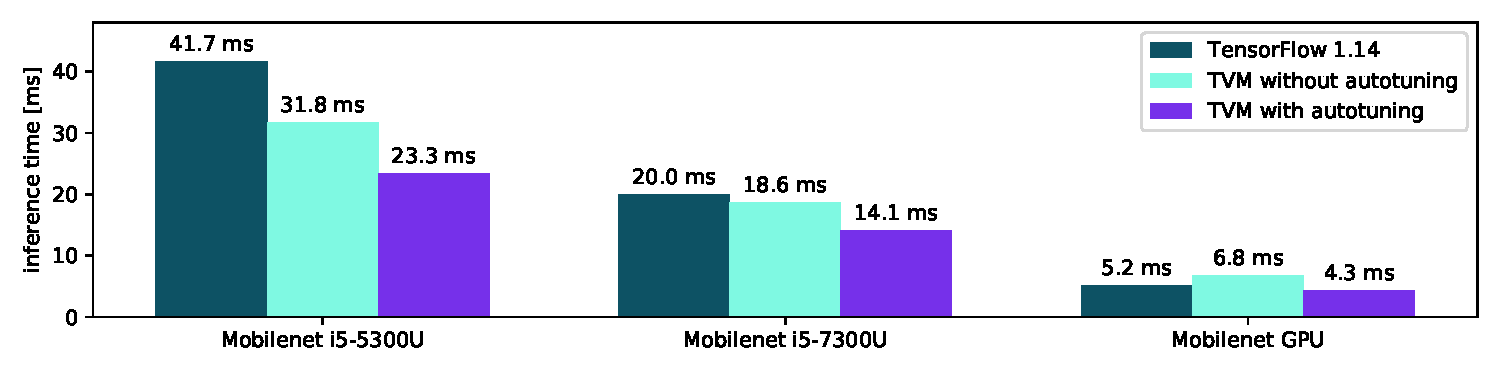
\includegraphics[width=\textwidth]{chart_inference_tf_vs_tvm}%
	\caption{Inference performance with TensorFlow and TVM}
	\label{fig:inf-tf-tvm}
\end{figure}

In all cases does TVM with autotuning show performance improvements over TensorFlow. Especially on CPU, inference takes 44\% (\SI{18.4}{\milli\second}) less time for the i5-5300U and 30\% (\SI{5.9}{\milli\second}) for the i5-7300U. For the server-grade CPU, inference takes 87\% (\SI{19.9}{\milli\second}) less time, presumably because TensorFlow is very slow due to the lack of SSE4 instructions, which TVM can much better cope with due to its flexibility. But also for the \gls{gpu}, the autotuned version takes 17\% (\SI{0.9}{\milli\second}) less time, albeit measurement inaccuracies are possible on this small scale. Nonetheless, even a similar performance is impressive considering that no human expert knowledge was required and autotuning took less than \SI{6}{\hour} for CPU and less than \SI{12}{\hour} for \gls{gpu} (due to the much larger search space). Further results for a wider variety of devices and models, including recurrent neural networks, are provided in \cite{Chen.2018} and show similar improvements.

TVM performs better than TensorFlow on CPU even without autotuning. Graph-level optimizations alone are enough to result in faster inference, taking 24\% (\SI{9.9}{\milli\second}) less time for the i5-5300U and 7\% (\SI{1.4}{\milli\second}) for the i5-7300U. Since only a series of pre-defined transformation passes are applied to the Relay program, graph-level optimization is performed in a matter of seconds. However, non-autotuned TVM cannot keep up with TensorFlow on GPU, it takes 31\% (\SI{1.6}{\milli\second}) longer.

These results show that TVM on par with manual optimization, at least for our limited evaluation scenarios. Furthermore, TVM is under active development and can be expected to show further performance improvements in the future.

\section{Limitations}
While the autotuning results are promising, we found that autotuning process suffers from some fundamental restrictions inherent to the current design which limit its efficiency. For all real measurements in this section, we evaluated autotuning of a ResNet-18 (12 convolutional layers, 1 fully-connected layer) with 2000 iterations per task on two machines with two Intel Xeon E5-2650 v3 CPUs and four Tesla K80 GPUs, one machine for client and target device each.

\subsection{Resource Utilization}
Since stages in autotuning depend on results of the previous stages (configurations are required for building, executables are necessary for profiling, time measurements are used to update the model), they need to be executed in sequence. Because profiling runs on the target device, the result is a lot of idle time on both the client and the target device. This sub-optimal \gls{resource}\footnote{We define \textit{resource} as a machine that executes some stage of the autotuning process, e.g., the target device or the hardware that the client runs on.} utilization is exemplified in Figure \ref{fig:tvm-res-util}.

\begin{figure}
	\centering
	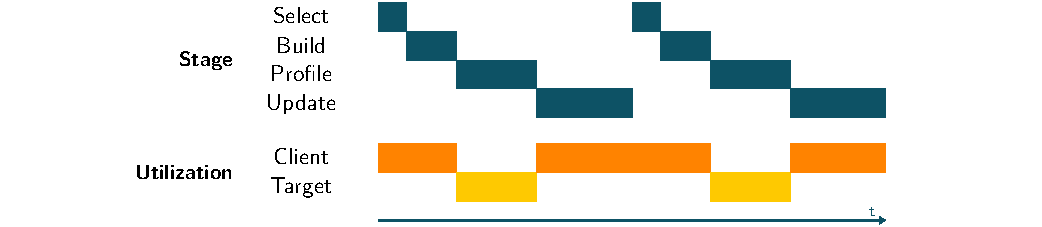
\includegraphics[width=\textwidth]{tvm_resource_utilization}%
	\caption{Resource utilization during autotuning}
	\label{fig:tvm-res-util}
\end{figure}

Measurements with our test setup showed that, for a total autotuning completion time of \SI{14.5}{\hour}, the client is idle for \SI{6.6}{\hour} (45\%) and the target device for \SI{7.9}{\hour} (55\%). Since computation resources, especially \gls{dl} accelerators, are rather costly, we want to minimize resource idle time. If existing resources are utilized better, it might not be necessary to acquire new hardware. If the individual occurences of idle time are long enough, it might be possible to use it for other computations in between. Indeed, the mean execution time for each stage is as follows: \SI{8.3}{\second} for building, \SI{39.5}{\second} for profiling, and \SI{44.0}{\second} for updating the model and selecting the next batch. This is long enough to reasonably assume that resource utilization can be improved by sharing the device. However, \gls{interference} must be prevented.

\subsection{Scalability}\label{sec:scalability}
In preparation for enabling autotuning on a larger-scale, we need to examine the scalability of the current design. Scalability in this section refers to the ability to run an arbitrary number of autotuning jobs at the same time without sacrificing efficiency and result quality. We define objectives, that a scalable solution should satisfy:
\begin{enumerate}
	\item High inference performance, since it is the ultimate goal of autotuning
	\item Low amount of required hardware, since additional devices are costly
	\item Low autotuning time, since autotuning takes long
\end{enumerate}
These objectives are listed in order of priority. Good inference performance is the primary objective. It obviates the need to buy new hardware. Furthermore, there usually is a large amount of inferences which makes a longer execution time for autotuning negligible in the long-term. Rapid autotuning is nonetheless desirable.

We compare two setups for scaling that are possible using only the components that TVM comes with by default, schematically depicted in Figure \ref{fig:tvm-scaling-setups}. For the sake of simplicity, we only show depict two jobs, but this generalizes to any higher number. The evaluation of both setups with regard to the previously defined objectives is summarized in Table \ref{tab:tvm-scaling-setups}.

\begin{figure}
	\begin{minipage}[b]{.45\textwidth}
		\centering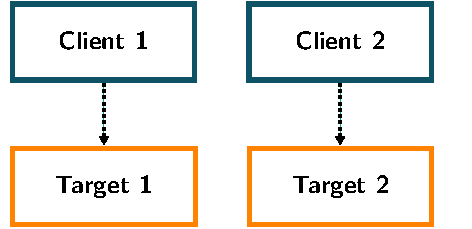
\includegraphics{scaling_setup_1}
		\subcaption{Dedicated resources}\label{fig:tvm-scaling-setups-1}
	\end{minipage}%
	\hspace{2em}
	\begin{minipage}[b]{.45\textwidth}
		\centering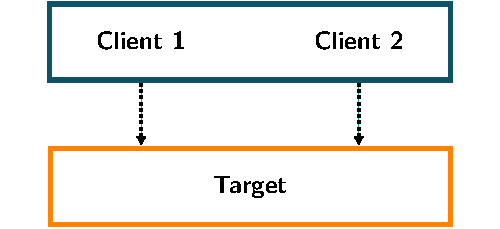
\includegraphics{scaling_setup_2}
		\subcaption{Shared resources}\label{fig:tvm-scaling-setups-2}
	\end{minipage}
	\caption{Setups for scaling autotuning}
	\label{fig:tvm-scaling-setups}
\end{figure}

\begin{description}
	\item[Dedicated resources] In the first setup (Figure \ref{fig:tvm-scaling-setups-1}), each job is run on its own set of resources. This means they are completely independent and do not affect each other. Both the resulting inference performance and the autotuning time are as good as possible, since they are equal to single-job autotuning. However, additional resources need to be acquired for every new job, which is not an economically feasible approach on a larger scale. Adding resources on demand from a cloud computing platform such as Amazon EC2 or Azure VM might work for the client machine, but since the actual target device needs to be used for profiling, which is likely to not be available on those cloud platforms, this is not a satisfactory solution. Alternatively to having separate sets of machines, the same machiens could be used to run the jobs in sequence. This trades off the amount of hardware that is required for autotuning time. With a higher number of jobs, this will take too long.
	\item[Shared resources] In the second setup (Figure \ref{fig:tvm-scaling-setups-2}), all jobs run in parallel on the same resource. To share the target device, we launch one RPC server for each client per GPU in our test setup. Due to the resource sharing, only one set of machines is required, which is good in terms of cost. However, this is very probable to lead to interference, when multiple jobs execute a stage on the same resource simultaneously. Interference has a detrimental effects on both inference performance and autotuning time. Interference on the client will slow down compute-intensive stages like building or model updates (50\%--70\% CPU usage). Modern CPUs are able to parallelize using multiple cores, but because building and model training uses all cores, time-sharing between multiple processes needs to be employed by the kernel. Process idle times and context switching overhead increase the autotuning time considerably. Assigning dedicated CPU cores per job will also make the process slower due to decreased resources per job and will not work when scaling up. Even more critical is interference on the target device. This distorts the profiling results, so good implementations might seem to perform bad if another job profiles on the same target device in parallel. Deceiving measurements will also lead to an inaccurate cost model. Since good inference performance is the prime objective of large-scale autotuning, this setup is also not satisfactory.
\end{description}

\begin{table}
	\newcommand\good[1]{\textcolor{hpe-green}{#1}}
	\newcommand\bad[1]{\textcolor{hpe-orange}{#1}}
	\newcommand\heading[1]{\textcolor{white}{\textbf{#1}}}
	\renewcommand{\arraystretch}{1.2}
	\sffamily
	\centering
	\begin{tabularx}{\textwidth}{l l l X}
	\rowcolor{black} \heading{Setup} & \heading{Hardware req.} & \heading{Inference speed} & \heading{Autotuning time} \vspace{2pt} \\
	\textbf{Dedicated resources} & \bad{2x} & \good{High} & \good{Low} \\
	\textbf{Shared resources} & \good{1x} & \bad{Low} & \bad{High} \\
	\textbf{Optimum} & \good{1x} & \good{High} & \good{Low} \\
	\end{tabularx}
	\caption{Comparison of scaling setups}
	\label{tab:tvm-scaling-setups}
\end{table}

Both setups do not meet all objectives we set for large-scale autotuning. Especially when scaling up to more parallel jobs, efficiency deteriorates significantly. We can conclude that the current implementation and architecture of autotuning in TVM does not scale well.

Having regarded possible scaling approaches and the reasons for their benefits and shortcomings, we can formulate two features for an optimal solution to satisfy the objectives:
\begin{itemize}
	\item Resources must be shared and utilized fully before adding new servers to minimize the required hardware for cost saving
	\item Interference must be prevented to guarantee a high inference performance and low autotuning time
\end{itemize}

\subsection{Similar Problems}
Our literature review was not successful in finding a solution to scale up autotuning. However, we can generalize the problem statement; we are looking for a solution to share available resources optimally between multiple tasks that are partially idle due to some dependency. From this point of view, we find two papers solving a similar problem.

\cite{Ma.2005} increases parallelism of a hierarchy of tasks and subtasks on multiprocessor platforms. Subtasks have control and data dependencies, but tasks are independent of each other. They employ a mix of exact and heuristic scheduling algorithms at design-time. Their scheduler interleaves sub-tasks of different tasks while respecting the dependencies between the subtasks of a single task. The result is a 37\% shorter execution time with increased resource utilization. The hierarchical structure of tasks and subtasks is similar to jobs and stages in autotuning.

\cite{Awatramani.2013} enable sharing of \gls{gpu} cores by multiple kernels. In current \gls{gpu} architectures, concurrently launched kernels use separate cores. However, interleaving of code from multiple kernels on the same core allows them to minimize core idle time introduced by memory latency. They increase the throughput of benchmarking applications by 7\%.

\cite{Ma.2005} and \cite{Awatramani.2013} improve parallelism for multiprocessing units while we want to improve parallelism for distributed machines. Nonetheless is the interleaving approach relevant.